\chapter{Application on Laplace's problem}
\label{ch:results}
\glsresetall

%Case 0: step-27
%\begin{align}
%  \Omega &= [-1,1]^d \setminus \left(-\frac{1}{2}, \frac{1}{2}\right)^d ,\\
%  - \nabla^2 u(\vec{x}) &= \prod\limits_{j=1}^{d} (x_j + 1) \quad\text{on}\quad \Omega,\\
%  u(\vec{x}) &= 0 \quad\text{on}\quad \partial\Omega
%\end{align}
%for $u$ scalar solution and $\vec{x} = (x_1, x_2, \dots, x_d)$ vector with $d$-components.

With all algorithms and data structures elaborated in Chs.~\ref{ch:parallel} and \ref{ch:dynamic}, we now have all features at our disposal to solve partial differential equations with parallel, dynamic \hp-adaptive \glspl{fem}. As a next step, we would like to apply our implementation in the \dealii{} library on a certain exemplary problem that showcases its error performance and parallel scalability. To quantify its capabilities, we want to find a scenario for which an analytic solution $u_\text{sol}$ is available allowing us to calculate the actual error of the finite element approximation. This approach for code verification corresponds to the method of manufactured solutions \parencite{salari2000}. Our choice for a suitable problem falls on solving the Laplace problem with Dirichlet boundary conditions:
\begin{align}
- \nabla^2 u(\vec{x}) &= 0 \quad\text{on}\quad \Omega \,\text{,} & u(\vec{x}) &= u_\text{sol}(\vec{x}) \quad\text{on}\quad \partial\Omega \,\text{.}
\end{align}

The choice to study the Laplace problem was not made by chance: We encounter the Laplace equation, or rather the Poisson equation with a non-vanishing right hand side, in many different modeling processes. In the field of electrostatics, the electric potential satisfies the Poisson equation. It is also used to model diffusion processes in time-dependent problems. Embedded in time discretization schemes, the Poisson problem has to be solved in each time step for, e.g., heat transfer problems. Further for the simulation of incompressible flows, the coupling of pressure and velocity is governed by the Poisson equation.

Following Eq.~\ref{eq:errorbound_hp}, we are aware that \p-adaptation is favorable in regions where the solution is regular, while \h-adaptation yields better results in regions with discontinuities or singularities. For elliptic problems like the Laplace one, we expect singularities on concave domains \parencite[Sec.~5.5]{brenner2008}.

\textcite{mitchell2014} presented several benchmarks for \hp-adaptation that make use of this observation. We decide to showcase our implementation on a two-dimensional domain with a reentrant corner located at the point of origin:
\begin{align}
\Omega &= \left\{ (r,\varphi) \in \mathbb{R}_{\geq 0} \times [0, 2 \pi) : (0 \leq r) \wedge( 0 \leq \varphi \leq \pi/\alpha) \right\} \,\text{,}
\end{align}
with $\alpha \in \left(1/2, 1\right)$. With the additional requirement that the solution must be zero along the legs of the reentrant corner, this particular scenario has a general solution which can be formulated in polar coordinates $r = \sqrt{x^2 + y^2} > 0$ and $\theta = \arctantwo(y,x)$:
\begin{align}
u_\text{sol}(\vec{x}) &= r^\alpha \sin(\alpha \, \theta) \,\text{,} \\
\nonumber \nabla u_\text{sol}(\vec{x}) &= \partial_r u_\text{sol}(\vec{x}) \vec{e}_r + \frac{1}{r} \partial_\theta u_\text{sol}(\vec{x}) \vec{e}_\theta \\
&= \alpha r^{\alpha - 1} \left[ \sin(\alpha \, \theta) \vec{e}_r + \cos(\alpha \, \theta) \vec{e}_\theta \right] \,\text{,}
\end{align}
with unit vectors \(\vec{e}_r = \cos(\theta) \vec{e}_x - \sin(\theta) \vec{e}_y\) and \(\vec{e}_\theta = \sin(\theta) \vec{e}_x + \cos(\theta) \vec{e}_y\). We immediately see that this solution has a singularity near the point of origin for the permitted values of $\alpha \in \left(1/2, 1\right)$:
\begin{align}
\left\| \nabla u_\text{sol}(\vec{x}) \right\|_{2} &= \alpha r^{\alpha - 1} \,\text{,} & \lim\limits_{r \rightarrow 0} \left\| \nabla u_\text{sol}(\vec{x}) \right\|_{2} &= \infty \quad\text{for}\quad \alpha \in \left(1/2, 1\right) \,\text{.}
\end{align}

In our testcase, we pick the corner to have a right angle with $\alpha = 2/3$ resulting in an L-shaped domain, at which all cells share the same topology to exclude influences from mesh distortion in our benchmark:
\begin{align}
\Omega_\text{L} &= \left[-1,1\right]^2 \setminus \left\{ \left(0,1\right) \times \left(-1, 0\right) \right\} \,\text{.}
\end{align}
A depiction of the solution on this particular domain is shown in Fig.~\ref{fig:solution}. The three dimensional variant of this problem is often referred to as the Fichera corner problem.

\begin{figure}
\centering
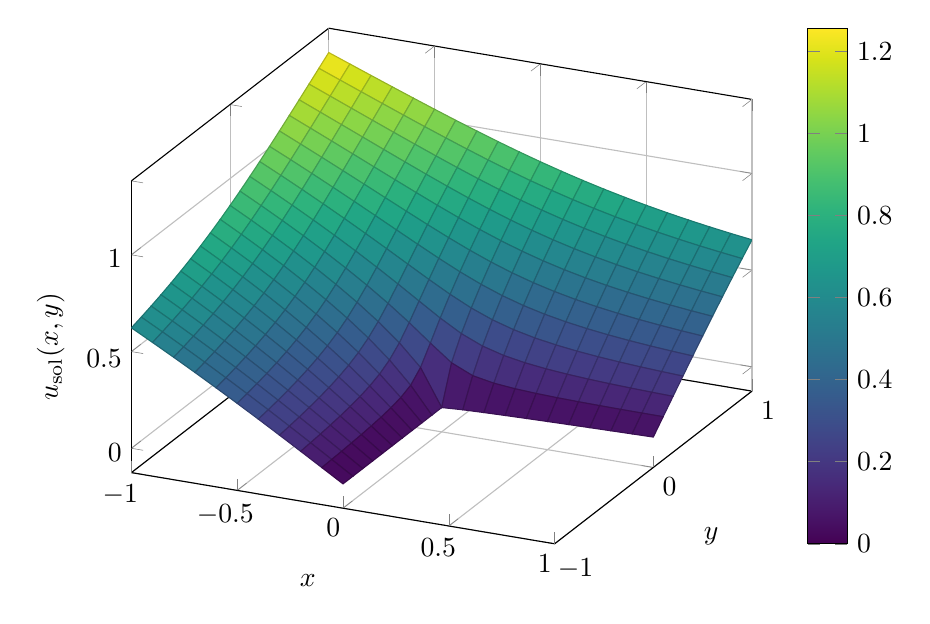
\begin{tikzpicture}
\begin{axis}[
  scale=1.15,
  surf,
  grid=major,
  colorbar,
  colormap/viridis,
  xlabel=$x$,
  ylabel=$y$,
  zlabel={$u_\mathrm{sol}(x,y)$}
  ]
\addplot3[
  surf,
  domain=-1:1,
  y domain=-1:1,
  restrict expr to domain={(x>0)&&(y<0)}{0:0},
  samples=21
  ]{pow(x*x+y*y,0.33)*sin(0.66*(atan2(y,-x)+90)))};
\end{axis}
\end{tikzpicture}%
\caption{Solution of the manufactured Laplace problem on a L-shaped domain.}
\label{fig:solution}
\end{figure}

In this chapter, we will solve the so designed Laplace problem on the L-shaped domain on consecutively refined meshes, and evaluate certain aspects of our implementation, namely the error performance of the decision strategies and their parallel scalability.

Following the usual approach in \gls{fem}, we transfer our problem to its weak formulation using \gls{cg} methods \parencite{brenner2008}:
\begin{align}
\left(\nabla u, \nabla v\right) &= 0 \,\text{,} & \forall v \in V &\coloneqq \left\{ v \in H^1(\Omega): v|_{\partial\Omega} = 0 \right\} \,\text{.}
\end{align}
The shape functions of Lagrangian elements will form the basis for the function space $V$. Dirichlet boundary conditions are imposed via constraints on \glspl{dof} located on the boundaries. The problem will be solved numerically with an iterative solver based on the conjugate gradient algorithm combined with an \gls{amg} preconditioner.

The \dealii{} library offers interfaces to parallel linear algebra of the third party libraries \petsc{} \textcite{petsc3124} and \trilinos{} \textcite{trilinos12181} for distributed memory architectures. In our investigations, we choose the latter using their \epetra{}
%\textcite{epetra}
module that handles all data infrastructure, and pick a corresponding solver from their \aztecoo{}
%\textcite{aztecoo}
package as well as their \ml{}
%\textcite{ml}
preconditioner. Compared to an equivalent configuration of \petsc{} modules, the \trilinos{} implementation yields more reproducible results using \gls{mpi} \parencite[FAQ]{petsc3124} and performs faster with higher order polynomials at more advanced refinement iterations according to our experience. For all calculations, we set a tolerance of $10^{-12}$ relative to the $l_2$-norm of the right hand side vector of the equation system.



\section{Error versus performance}
\label{sec:errorvsperformance}

%Global H1 error as measure
%\begin{align}
%\| e_{hp} \|_{H^1(\Omega)}^2 &= \sum\limits_K \| e_{hp} (\vec{x}) \|_{H^1(K)}^2 \\
%\| e_{hp} \|_{H^1(K)}^2 &= \int_K (|e_{hp}|^2 + |\nabla e_{hp}|^2) \differential{\vec{x}}
%\end{align}
%with error function $e_{hp} = u - u_{hp}$.

% setup of scenario

The main motivation of \hp-adaptive methods are their superior error convergence characteristics compared to the more common \h-adaptive ones provided that the solution is sufficiently regular. We will demonstrate their advantages on our presented scenario and use consecutively adapted meshes to illustrate their error performance in relation to their workload on the numerical example.

%Demonstrate adaptive algorithms , and how the error reduces with.
%compare error with the workload either measured in the number of \glspl{dof} or the actual wall time. % maybe later

The consecutively adapted meshes so created are by far not optimal for the problem, nor is finding such an optimal mesh subject of this dissertation. We are rather interested in comparing the performance and results of the decision algorithms presented in Sec.~\ref{sec:decision}, and whether they are capable of localizing regions with singularities, i.e.\@ the one at the point of origin for our numerical example. We will compare all types of adaptation at our disposal, i.e.\@ \h-, \p-, and \hp-adaptation. For the latter, we examine all three presented strategies in contrast, namely error prediction and smoothness estimation by either Legendre or Fourier coefficient decay.

After solving the linear equation system in each step and calculating the error on basis of the analytic solution according to \textcite{kelly1983}, we use the \textit{fixed-number} strategy to indicate adaptation: The 30\% fraction of all cells with the highest error will be flagged for refinement, and 3\% of those with the lowest error will be marked for coarsening. This allows us to compare the results of each adaptation type under the same conditions, since always the same amount of cells is going to be changed. The idea behind additional coarsening is motivated by the fact that we tend to refine too many cells with error estimators providing an upper bound for the error, or error indicators based on heuristics. We would like to correct this from a previous iteration by coarsening a small amount of cells. The combination of fractions of 30\% for refinement and 3\% for coarsening has become a reasonable choice for two-dimensional applications within the \dealii{} library.

%We will compared different refinement strategies. We will use \textit{fixed-fraction} adaptation so that every cell is refined. This allows us to compare the choices of all strategies since always the same amount of cells is taken into account. \todo{see slack text}

Further for \hp-adaptive strategies, we need to choose a decision strategy providing corresponding indicators that propose which type of adaptation we want to impose one each cell.
%
Again, we use the \textit{fixed-number} algorithm on all decision indicators. This allows us to compare the choices made by each strategy since always the same amount of cells is going to be changed in terms of both \h- and \p-adaptation, respectively.
%
As a first naive approach, we will impose the \h-variant on one half of all cells previously marked for adaptation, and the \p-variant on the other half.
%As a first naive approach, we choose between \h- and \p-adaptation fifty fifty among all cells that have been previously marked for adaptation.
%, based on the specified decision criterion.
As a second attempt, since we know that we have only one single localized and well-defined singularity in the domain, we are confident to make an educated guess and assign 90\% of flagged cells for \p- and the remaining 10\% for \h-adaptation. From here, we refer to the first approach if we call a decision strategy naive, and speak of the second if no such attribute was given.

To setup the numerical example, we start with a mesh consisting of three cells as the coarsest possible representation of our L-shaped domain, which will be globally refined five times to form the initial grid for all investigations in this section.

The error prediction strategy forms an exception since it requires a prepended initialization step. In this case, we will begin with four initial refinement steps, solve the equation system, and perform another global refinement so that we have the corresponding prediction available. Further for this strategy, control parameters are set to $\gamma_n = 1$, $\gamma_h = 1$, and $\gamma_p = \sqrt{0.4}$, which corresponds to the values used by \textcites{melenk2001}{mitchell2014}.

We use a collection of Lagrangian finite elements $Q_p$ with polynomial degrees $p \in [2,7]$ and skip linear elements due to our observation that the smoothness estimation algorithms perform poorly with those. All cells will be initially assigned with the lowest order element. In the case of sole \h-adaptation, all elements will be assigned to $Q_2$ elements. For pure \p-adaptation, we favor \p-adaptation to \h-adaptation as long as the finite element can be \p-adapted, i.e.\@ the current finite element is neither at the top nor the bottom of the hierarchy. We perform a total of twelve consecutive adaptation iterations, so twice as many as there are different finite elements.

All calculations in this section have been carried out on a desktop machine, using an Intel \todo{trademark} Core i7-4790 processor running at 3.6 GHz with 32 GB of memory \todo{si}. Although this is a quad-core processor offering a total of eight threads utilizing hypertreading, we will only use a single thread for our calculations, which is sufficient to determine both error and workload. We will deal with parallelization in later sections.


% results: error vs ndofs

Representatively, we will show the grid and distribution of finite elements after six adaptation cycles of the Legendre coefficient decay strategy with the educated guess approach in Fig.~\ref{fig:fedegrees}. All other meshes after equally many adaptation iterations from the other strategies are showcased in App.~\ref{app::strategies}.

We see that the Legendre strategy is able to locate the singularity in the center by preferring \h-adaptive refinement in this section, while using \p-adaptation in the other regions. This is also the case for all other strategies, naiive or not, as shown in App.~\ref{app::strategies}.

\begin{figure}
\centering
Insert distribution of finite elements for Legendre strategy after five iterations.
\caption{Distribution of finite elements after five iterations with the Legendre coefficient decay strategy.}
\label{fig:fedegrees}
\end{figure}

We will plot the $H_1$ error against the workload, which can be measured in two ways: Either with the number of \glspl{dof}, or the elapsed real time from start to end of our application, which we refer to as wall time. We begin with identifying the workload with the former and show corresponding results in Fig.~\ref{fig:errordofs}.

%We measure the workload in two different ways and present the results separately. First, with the number of \glspl{dof} for each individual iteration, and second, with the total wall time accumulated over the current and all previous iterations.

\begin{figure}
\begin{subfigure}{1\textwidth}
  \centering
  \begin{tikzpicture}
\begin{loglogaxis}[
  xlabel=Number of \glspl{dof},
  ylabel=H1 error]
\addplot table [y=H1 error, x=ndofs, col sep=comma] {data/error/h.csv};
\addplot table [y=H1 error, x=ndofs, col sep=comma] {data/error/p.csv};
\addplot table [y=H1 error, x=ndofs, col sep=comma] {data/error/hp-legendre.csv};
\addplot table [y=H1 error, x=ndofs, col sep=comma] {data/error/hp-fourier.csv};
\addplot table [y=H1 error, x=ndofs, col sep=comma] {data/error/hp-prediction.csv};
\addplot table [y=H1 error, x=ndofs, col sep=comma] {data/error/hp-legendre-naive.csv};
\addplot table [y=H1 error, x=ndofs, col sep=comma] {data/error/hp-fourier-naive.csv};
\addplot table [y=H1 error, x=ndofs, col sep=comma] {data/error/hp-prediction-naive.csv};
\end{loglogaxis}
\end{tikzpicture}
  \caption{Double logarithmic representation. The thick line corresponds to the reference Eq.~(\ref{eq:errorbound_ana}).}
  \label{fig:errordofsloglog}
\end{subfigure}
\begin{subfigure}{1\textwidth}
  \centering
  \begin{tikzpicture}
\begin{semilogyaxis}[
%  scale only axis,
  xlabel=Number of \glspl{dof},
  ylabel=H1 error,
  legend pos=outer north east]
%\addplot table [y=H1 error, x=ndofs, col sep=comma] {data/error/h.csv};
%\addlegendentry{\h};

\addplot table [y=H1 error, x=ndofs, col sep=comma, select coords between index={0}{5}] {data/error/p.csv};
\addlegendentry{\p};

\addplot table [y=H1 error, x=ndofs, col sep=comma, select coords between index={0}{5}] {data/error/hp-legendre.csv};
\addlegendentry{\hp{}-Legendre};

\addplot table [y=H1 error, x=ndofs, col sep=comma, select coords between index={0}{5}] {data/error/hp-fourier.csv};
\addlegendentry{\hp{}-Fourier};

\addplot table [y=H1 error, x=ndofs, col sep=comma, select coords between index={0}{6}] {data/error/hp-prediction.csv};
\addlegendentry{\hp{}-prediction};

%\addplot table [y=H1 error, x=ndofs, col sep=comma] {data/error/hp-legendre-naive.csv};
%\addlegendentry{\hp{}-Legendre naive};
%
%\addplot table [y=H1 error, x=ndofs, col sep=comma] {data/error/hp-fourier-naive.csv};
%\addlegendentry{\hp{}-Fourier naive};
%
%\addplot table [y=H1 error, x=ndofs, col sep=comma] {data/error/hp-prediction-naive.csv};
%\addlegendentry{\hp{}-prediction naive};

%\addplot[very thick, samples=100, domain=10000:50000] {10^(-2)*exp(10^(-3.9)*(-x+10000))}; % {10^(-4)*(-x+10000)};
\end{semilogyaxis}
\end{tikzpicture}
  \caption{Customly scaled coordinate system with the y-axis scaled exponentially and the x-axis scaled with the cubic root. The thick line corresponds to the reference Eq.~(\ref{eq:errorbound_exp}) with $b = 0.18$.}
  \label{fig:errordofscustom}
\end{subfigure}
\caption{Error vs workload.}
\label{fig:errordofs}
\end{figure}

The double logarithmic representation of our results in Fig.~\ref{fig:errordofsloglog} reveals analytic convergence for the \h-adaptive case, but at a lower rate as presented in Eq.~(\ref{eq:errorbound_ana}), which translates to $n_\text{dofs}^{-1}$ in our scenario. An explanation would be that we are not working with quasiuniform but rather highly adapted meshes.

Eq.~(\ref{eq:errorbound_exp}) predicts exponential decay for \hp-adaptive strategies, which we would like to verify in Fig.~\ref{fig:errordofscustom} with a customly scaled plot featuring a logarithmic y-axis and an x-axis scaled with the cubic root, which corresponds to the correct exponent in our numerical example. Indeed, we see exponential convergence in the \p-adaptive and \hp-adaptive strategies to the proclaimed rate, however the naive approaches miss it. Thus a high proportion of \p-refinement is required to yield exponential decay in this scenario.

The \p-strategy shows a similar decay as the \hp-adaptive methods.%, but the error in the last cycle is still by a factor of two higher.
In this strategy, \p-refinement will be applied up to the point until it is no longer possible after we reached the highest order element in the hierarchy. With six distinct finite elements in our collection, we will apply \h-refinement for the first time after the sixth data point, at which a major drop is observable. We also see that the exponential decay proclaimed in Eq.~(\ref{eq:errorbound_exp}) is only observable after applying \h-refinement. Thus, we conclude that \h-refinement is mandatory to reduce the error to the observed low order of magnitude.

To solve the equation system in the last adaptation cycle, the \hp-adaptive methods %corresponding to our educated guess 
srequire a number of \glspl{dof} by a factor of 100 less than the \h-adaptive methods to reach the same accuracy
%need a factor of 1,000 less \gls{dof} to reach the same accuracy as the \h-adaptive methods
and by factor of 10 less compared to their naive counterparts. This demonstrates that \hp-adaptive methods are the methods of choice for this particular scenario.

%We conclude that \p-heavy refinement combined with \h-adaptation near the singularity perform the best error per workload ratio.

In the course of adaptation with the Fourier strategy, some adaptation steps increase the number of \gls{dof} without decreasing the error, which we refer to as 'hickups'.
%We see certain outliers in the plots for Fourier strategy.
We observed that they occur if the finite element with the highest polynomial degree in our mesh increases from fourth to fifth order. This is perhaps not a causal relation, and we have not yet found the reason for these 'hickups'.

%Compared to \h- and naive \hp-approaches, \p- and \hp-strategies featuring the educated guess yield similar results.

%We reach about one order of magnitude lower errors with \hp-adaptive strategies compared to the \p-adaptive, which might be due to the singularity that the latter does not resolve \todo{?}.


% results: error vs walltime

From a practical point of view, the error performance will now be compared to the actual wall time to measure whether we have an economic benefit in using \hp-adaptive methods. For each consecutive adaptation cycle, we again plot the calculated error against the workload, which is this time represented by the total run time accumulated over the current and all previous iterations. Each run will be repeated five times and the minimum over the total runtime over all runs will be picked to compensate for temporarily high loads on memory bandwidth. The results are shown in Fig.~\ref{fig:errorwalltime}.

\begin{figure}
%\begin{subfigure}{1\textwidth}
\centering
\begin{tikzpicture}
\begin{loglogaxis}[
  xlabel=Wall time {[seconds]},
  ylabel=H1 error,
  legend pos=outer north east]
\addplot table [y=H1 error, x=walltime, col sep=comma] {data/error/h.csv};
\addlegendentry{\h};

\addplot table [y=H1 error, x=walltime, col sep=comma] {data/error/p.csv};
\addlegendentry{\p};

\addplot table [y=H1 error, x=walltime, col sep=comma] {data/error/hp-legendre.csv};
\addlegendentry{\hp{}-Legendre};

\addplot table [y=H1 error, x=walltime, col sep=comma] {data/error/hp-fourier.csv};
\addlegendentry{\hp{}-Fourier};

\addplot table [y=H1 error, x=walltime, col sep=comma] {data/error/hp-prediction.csv};
\addlegendentry{\hp{}-prediction};

\addplot table [y=H1 error, x=walltime, col sep=comma] {data/error/hp-legendre-naive.csv};
\addlegendentry{\hp{}-Legendre naive};

\addplot table [y=H1 error, x=walltime, col sep=comma] {data/error/hp-fourier-naive.csv};
\addlegendentry{\hp{}-Fourier naive};

\addplot table [y=H1 error, x=walltime, col sep=comma] {data/error/hp-prediction-naive.csv};
\addlegendentry{\hp{}-prediction naive};
\end{loglogaxis}
\end{tikzpicture}
%  \caption{Error vs workload.}
%  \label{fig:errorexpworkload}
%\end{subfigure}
%\begin{subfigure}{1\textwidth}
%  \centering
%  \begin{tikzpicture}
\begin{semilogyaxis}[
  xlabel=Wall time {[seconds]},
  ylabel=H1 error,
  legend pos=outer north east]
%\addplot table [y=H1 error, x=walltime, col sep=comma] {data/error/h.csv};
%\addlegendentry{\h};

\addplot table [y=H1 error, x=walltime, col sep=comma, select coords between index={0}{5}] {data/error/p.csv};
\addlegendentry{\p};

\addplot table [y=H1 error, x=walltime, col sep=comma, select coords between index={0}{5}] {data/error/hp-legendre.csv};
\addlegendentry{\hp{}-Legendre};

\addplot table [y=H1 error, x=walltime, col sep=comma, select coords between index={0}{5}] {data/error/hp-fourier.csv};
\addlegendentry{\hp{}-Fourier};

\addplot table [y=H1 error, x=walltime, col sep=comma, select coords between index={0}{6}] {data/error/hp-prediction.csv};
\addlegendentry{\hp{}-prediction};

%\addplot table [y=H1 error, x=walltime, col sep=comma] {data/error/hp-legendre-naive.csv};
%\addlegendentry{\hp{}-Legendre naive};
%
%\addplot table [y=H1 error, x=walltime, col sep=comma] {data/error/hp-fourier-naive.csv};
%\addlegendentry{\hp{}-Fourier naive};
%
%\addplot table [y=H1 error, x=walltime, col sep=comma] {data/error/hp-prediction-naive.csv};
%\addlegendentry{\hp{}-prediction naive};

%\addplot[very thick, samples=100, domain=0.1:5] {10^(-2)*exp(10^(0)*(-x+0.1))}; % {10^(-4)*(-x+10000)};
\end{semilogyaxis}
\end{tikzpicture}
%  \caption{Error vs walltime.}
%  \label{fig:errorexpwalltime}
%\end{subfigure}
\caption{Double lagarithmic error vs walltime.}
\label{fig:errorwalltime}
\end{figure}

%We notice that the choice of the \hp-adaptive strategy has an impact on the error performance compared to the number of \glspl{dof}. However in comparing error with the runtime, we see that all methods perform similarly. We will postpone the discussion on this topic for the later Sec.~() in which we give an in-depth analysis on the sacalability of certain parts of our code, in which we think to identify the reason for this behavior.

Again after the last adaptation cycle, \p- and \hp-adaptive methods are most efficient and about an order of magnitude faster than the \h-adaptive variant. Interestingly, the wall times of the naive \hp-strategies fan out. It appears that a high diversity of finite elements compared with major grid adaptation increase the wall time significantly, and we suspect that the combination of solver and \gls{amg} preconditioner is responsible for this behavior. We will discuss this topic later in the scalability analysis.

The Fourier strategy takes the longest wall time for initialization, during which the Fourier transformation matrices are calculated. This is a costly operation, which requires substantially more quadrature points during calculation than the Legendre equivalent, and is responsible for the observable offset.

% this is general observation
Among all \hp-strategies of either naive or educated guess category, we do not see major differences in their performance, but overall the Legendre coefficient decay strategy stands out in both categories with the best error per workload performance in either way workload is defined.
%Compared to the Fourier strategy, it seems to be better suited for \gls{fem} since its basis functions are also based on polynomials.

% write this in the next chaper
%In the upcoming scalability analysis, we will thus pick this strategy with Legendre coefficient and the educated guess.

%Overall, the Legendre coefficient strategy yields the best error per workload performance in both categories.

%Again, to mitigate the impact of temporary slowdowns on the supercomputer due to a high loads on memory and network bandwidth, we repeat each run for a total of \todo{five?} times and take the minimal runtime in each category over all runs.
\section{Load balancing heuristics}
\label{sec:heuristics}

% introduction

For parallel computations on distributed memory systems, the global domain is partitioned into several subdomains, each of which is assigned to a single process. Such a mesh decomposition is showcased in Fig.~\ref{fig:decomposition}.

\begin{figure}
\centering
\begin{subfigure}[t]{.49\textwidth}
  \centering
  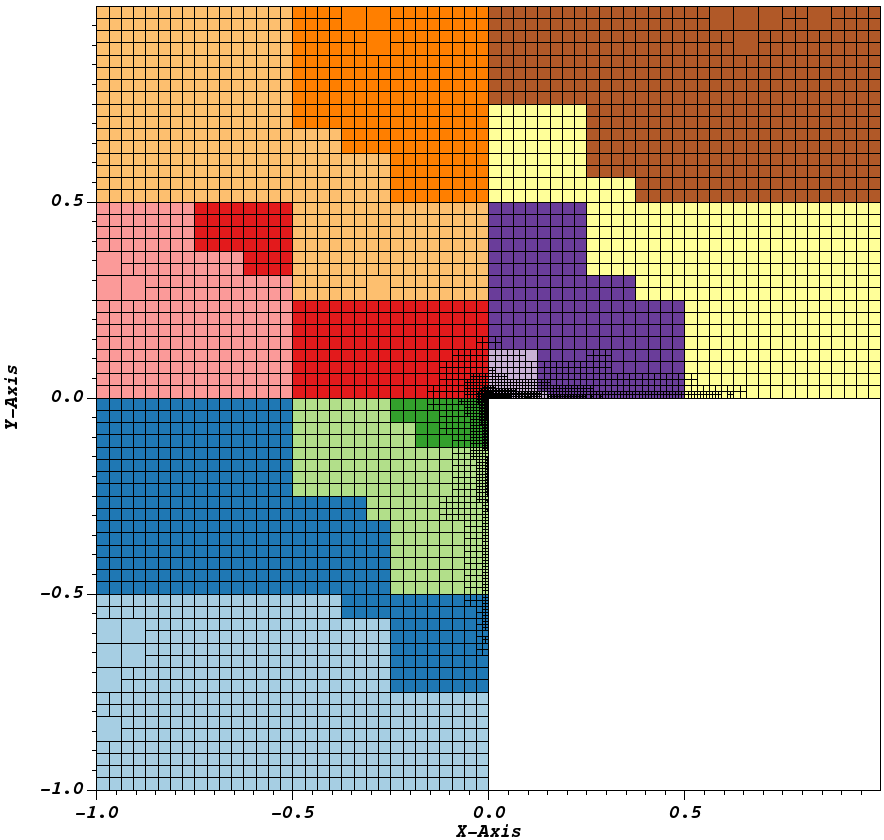
\includegraphics[width=\textwidth]{figures/results/corner-2d-error-hp-legendre-05_subdomain12.png}
  \caption{Constant weighting.}
\end{subfigure}
\begin{subfigure}[t]{.49\textwidth}
  \centering
  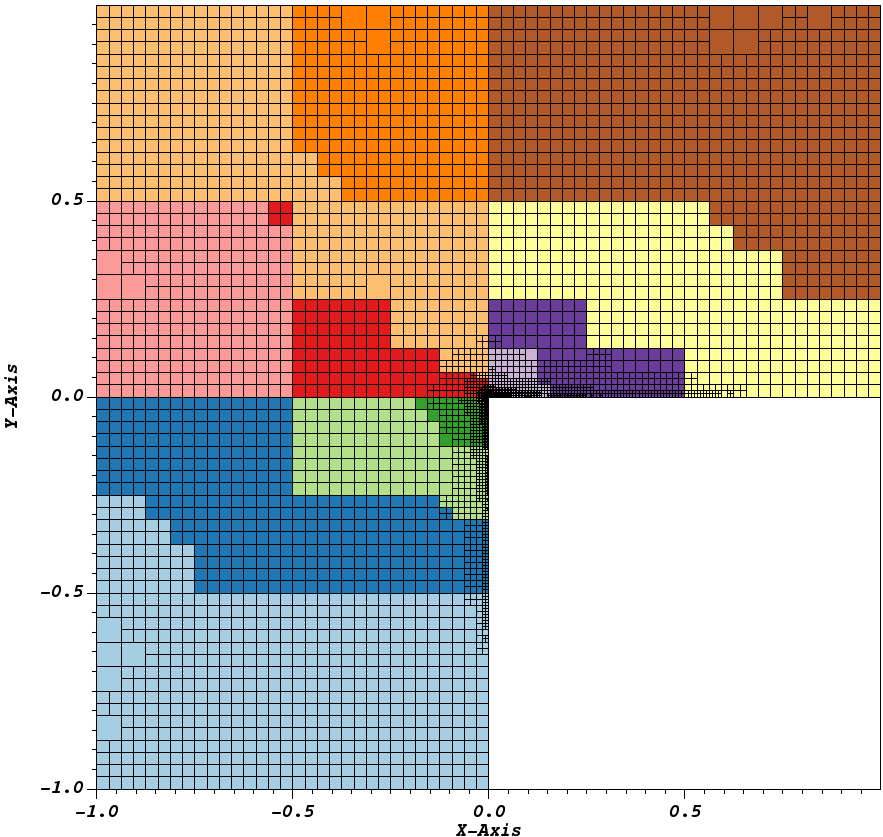
\includegraphics[width=\textwidth]{figures/results/corner-2d-error-hp-legendre-05_subdomain12_customweighting.png}
  \caption{Weighting with an individually potentiated number of \glspl{dof}, i.e.\@ $\propto n_\text{dofs}^{1.9}$.}
\end{subfigure}
\caption{Decomposition of the mesh after six iterations with the Legendre coefficient decay strategy on 12 \gls{mpi} processes with various cell weighting. Each color represents a different subdomain.}
\label{fig:decomposition}
\end{figure}

Proper load balancing is necessary for an efficient use of all computational resources. Especially on \gls{hpc} systems with lots of available processors, this is a critical feature. For \hp-adaptive \gls{fem}, we presented approaches for load balancing in Sec.~\ref{sec:loadbalancing} by assigning weights to each individual cell and balancing the accumulated weight among all processes. We relate the weight to the number of \glspl{dof} on each cell potentiated by an exponent that we will determine in the upcoming investigations. Or in other words, cell weights are chosen proportional to $n_\text{dofs}^c$ with the exponent $c$ to be ascertained.

Although all three \hp-adaptive strategies have demonstrated a similar performance as shown in Sec.~\ref{sec:errorvsperformance}, we pick only one adaptation strategy for our parallel investigations. We choose the smoothness estimation strategy based on the decay of Legendre coefficients as the most efficient one for this purpose.

% system specifications

Investigations are carried out on the JURECA supercomputer \parencite{krause2016}. Each computing node is equipped with two Intel\textsuperscript{\textregistered} Xeon\textsuperscript{\textregistered} E5-2680 v3 processors with twelve cores running at 2.5GHz and either 128GB, 256GB or 512GB of memory. With simultaneous multithreading, a total of 48 threads are available per node. Communication between nodes happens via a Mellanox EDR InfiniBand high-speed network.

In this section, our investigations are performed on two distinct nodes, which provide a total of 96 threads and involve communication between two physically independent memory segments. We expect that this setup yields representative results that can be extrapolated on even larger problem sizes.

Further, we use a 'flat' \gls{mpi} model: Every thread will be assigned to an individual \gls{mpi} process and no additional thread parallelization is invoked. Although \dealii{} provides such a feature via Intel\textsuperscript{\textregistered} \gls{tbb}, we refrain from using it to measure the pure \gls{mpi} performance for all parallel analyses in this dissertation.

% problem specifications

To qualify our problem for parallel computations, we need to increase its size drastically. The problem is initialized with nine global refinements and gets adapted in twelve iterations. For the strategy with the Legendre coefficient decay, this results in a total number of 46,369,440 \glspl{dof}, so that in the best case each process will be assigned to a number of 483,015 \glspl{dof} on average. Each type of finite element from the provided collection is represented at least once in the mesh.

This advanced scenario will form the basis of our investigations to see how different weighting exponents affect the wall time, and which one provides a minimum. With serialization, we ensure that each of these runs conforms to the same conditions. Again, to mitigate the impact of temporary slowdowns on the supercomputer due to high loads on memory and network bandwidth, we repeat each run for a total of five times and take the minimum wall time in each category over all runs.

% results

For varying weighting exponents, we compare the wall times of the full adaptation cycle and its relevant sections
%For resumed scenarios in which the mesh will be partitioned according to weights with different weighting exponents, we compare the wall time of critical sections of the program as well as the total wall time
%between runs with different weighting exponents
in Fig.~\ref{fig:weights}.

\todo{Second scale for assembly/discontinued axis with groupplot}
%https://tex.stackexchange.com/questions/46422/axis-break-in-pgfplots
\todo{Maybe also add setup of data structure and other parts}
\begin{figure}
\centering
\begin{tikzpicture}
\begin{axis}[
  xlabel=Weighting exponent,
  ylabel=Wall time {[seconds]},
  legend pos=outer north east]

\addplot table [y=full cycle, x=weighting exponent, col sep=comma] {data/weight/weight.csv};
\addlegendentry{full cycle};

\addplot table [y=assembly, x=weighting exponent, col sep=comma] {data/weight/weight.csv};
\addlegendentry{assemble linear system};

\addplot table [y=solve, x=weighting exponent, col sep=comma] {data/weight/weight.csv};
\addlegendentry{linear solver and preconditioner};
\end{axis}
\end{tikzpicture}
\caption[Wall times for load balancing with varying weighting exponents.]{Wall times of a complete adaptation cycle and those parts relevant for load balancing. The problem has a number of about 46 million \glspl{dof} and is solved on 2 nodes or 96 \gls{mpi} processes. Weights proportional to $n_\text{dofs}^c$ will be assigned to each cell with varying exponents $c$.}
\label{fig:weights}
\end{figure}

As discussed in Sec.~\ref{sec:balancing}, the assembly of the equation system and the its solution are identified as the critical sections whose wall time is affected by the number of \glspl{dof}. We see that the solution of the equation system takes about 90\% of the total wall time and is the crucial factor for proper load balancing. The minimal wall time for both solver and the full cycle is reached with a weighting exponent of $c = 1.9$.

We were surprised to find the minimum wall time of the solver at such a high exponent, since we expected $c = 1$ for an efficient solver. This may be related to the implementation of the preconditioner combined with the disorder that \hp-adaptive methods cause in the system matrix. Further, we were expecting a minimum in the assembly at about $c = 2$, but found it was decaying at even higher exponents. We have no explanation for this behavior. Analyzing the effect of cell weighting on each individual section of the program
%the load balancing
will be subject of further investigations.

% Next step
%We set an weighting expoenent to a value of $c = 1.9$ for the following considerations regarding scalability.

\section{\Glsfmtlong{hpc} scalability}
\label{sec:scaling}

The final part of our investigations relates to the demonstration of the scalability of our algorithms and data structures on \gls{hpc} systems, for which we will again use the JURECA supercomputer \parencite{krause2016}.

Again working with successively adapted meshes, we will measure the wall time spent in each particular section of each SOLVE-ESTIMATE-MARK-REFINE iteration, which is supposed to increase linearly with the workload determined by the number of \glspl{dof} or decrease linearly with an increasing amount of workers, i.e.\@ number of \gls{mpi} processes. We distinguish between the following categories in each adaptation cycle similar to \textcite{bangerth2012}:
\begin{itemize}
\item \textit{Setup data structures}. Enumerate all \glspl{dof}. Determine the sparsity pattern describing locations of nonzero matrix entries. Calculate constraints for hanging nodes and boundary values. Allocate memory for all distributed data structures. Communicate between processes which matrix or vector elements they will write to that they do not own locally.
\item \textit{Assemble linear system}. Calculate the individual contribution of each locally owned cell to the global equation system. Exchange data if matrix or vector elements are stored on a different process.
\item \textit{Linear solver and preconditioner}. Setup both the \gls{amg} preconditioner and the conjugate gradient solver and solve the equation system in parallel.
\item \textit{Estimate error}. Calculate the error indicators on locally owned cells on basis of the current solution. Mark cells for either refinement or coarsening by computing global thresholds.
\item \textit{Estimate smoothness}. Calculate the smoothness indicators on basis of the current solution on locally owned cells marked for either refinement or coarsening. Decide whether \h- or \p-adaptation is going to be applied by computing global thresholds.
\item \textit{Coarsen and refine}. Perform coarsening and refinement and maintain the 2:1 cell balance on the \pforest{} master mesh, followed by its repartitioning. Transfer data between the outdated and updated mesh. Apply all changes made to the master mesh on the \dealii{} triangulation.
\end{itemize}

We will pick the parameters and features that have proven to be suitable in our numerical example. Thus, we again choose smoothness estimation by the decay of Legendre coefficients as our \hp-decision strategy. For load balancing, cell weighting is imposed proportional to the number of \glspl{dof} on each cell potentiated by the exponent $c = 1.9$.


% weak scaling

For weak scaling, problems with increasing size are solved on a fixed number of \glspl{mpi} processes, which we will realize using consecutive adaptations. We choose two different numbers of computation nodes, namely 16 and 64 nodes with 768 and 3,072 \glspl{mpi} processes in total each.

We initialize the problem with ten initial global refinements and adapt the mesh for a total of 11 iterations with the smaller amount of computing nodes, and 12 iterations for the larger one. In the chosen configuration, all available memory is used on the assigned nodes, so no more adaptation cycles are possible without running out of memory. Again to exclude the influence of the current load on the supercomputer, all runs are performed multiple times and the minimum wall time of each category is taken. This time we repeat each run seven times. The results of weak scaling are shown in Fig.~\ref{fig:weak} up to problem sizes of 2,073,075,769 \glspl{dof}.

\begin{figure}
\begin{subfigure}{1\textwidth}
  \centering
  \begin{tikzpicture}
\begin{loglogaxis}[
  xlabel=Number of \glspl{dof},
  ylabel=Wall time {[seconds]},
  legend pos=outer north east]

% data
\addplot table [y=solve, x=ndofs, col sep=comma] {data/weak/weak-nodes16.csv};
\addlegendentry{linear solver and preconditioner};

\addplot table [y=setup, x=ndofs, col sep=comma] {data/weak/weak-nodes16.csv};
\addlegendentry{setup data structures};

\addplot table [y=assembly, x=ndofs, col sep=comma] {data/weak/weak-nodes16.csv};
\addlegendentry{assemble linear system};

\addplot table [y=compute errors, x=ndofs, col sep=comma] {data/weak/weak-nodes16.csv};
\addlegendentry{estimate error};

\addplot table [y=calculate indicators, x=ndofs, col sep=comma] {data/weak/weak-nodes16.csv};
\addlegendentry{estimate smoothness};

\addplot table [y=refine, x=ndofs, col sep=comma] {data/weak/weak-nodes16.csv};
\addlegendentry{coarsen and refine};

% optimal line
\addplot[very thick, samples=2, domain=12591105:1302365268] {10^(-7.2)*x};
\addlegendentry{optimal convergence};

% auxiliary lines
\begin{scope}
  \draw[green] ({axis cs:76800000,0}|-{rel axis cs:0,1}) -- ({axis cs:76800000,0}|-{rel axis cs:0,0});
  \draw[blue] ({axis cs:50647318,0}|-{rel axis cs:0,1}) -- ({axis cs:50647318,0}|-{rel axis cs:0,0});
\end{scope}
\addlegendimage{color=green};
\addlegendentry{$10^5$ \glspl{dof} per process};
\addlegendimage{color=blue};
\addlegendentry{each finite element in mesh};
\end{loglogaxis}
\end{tikzpicture}%
  \caption{Weak scaling on 16 nodes or 768 \gls{mpi} processes.}
  \label{fig:weak-nodes16}
\end{subfigure}
\begin{subfigure}{1\textwidth}
  \centering
  \begin{tikzpicture}
\begin{loglogaxis}[
  xlabel=Number of \glspl{dof},
  ylabel=Walltime {[seconds]}]

\addplot table [y=full cycle, x=ndofs, col sep=comma] {data/weak/weak-nodes64.csv};

\addplot[very thick, samples=2, domain=12591105:2073075769] {10^(-3)*x};

\end{loglogaxis}
\end{tikzpicture}%
  \caption{Weak scaling on 64 nodes or 3,072 \gls{mpi} processes.}
  \label{fig:weak-nodes64}
\end{subfigure}
\caption{Weak scaling for consecutively refined meshes on different numbers of \glspl{mpi} processes. Each \gls{mpi} process has more than $10^5$ \glspl{dof} assigned only to the right side of the indicated vertical line. Each finite element is represented at least once in the mesh only to the right side of the designated vertical line.}
\label{fig:weak}
\end{figure}

\textcite{bangerth2012} proclaimed that linear scaling is observable in all categories if the number of \glspl{dof} per \gls{mpi} process exceeds $10^5$. We can confirm this observation in our numerical example with parallel \hp-adaptation as well.

During the first few adaptation cycles in our application, the wall time attributed to the solution category shows a major increase which is much more than just linear. After six adaptation cycles, i.e.\@ right of the indicated vertical line in Fig.~\ref{fig:weak}, each finite element will be represented at least once in the domain due to the way we configured the scenario, and the aforementioned curve flattens and increases only linearly as expected.

%We suspect that the randomness of the distribution of 

%We suspect that the mixture of many different finite elements are the reason for this behavior

%that adding finite elements of a higher order than before results in a higher complexity in the matrix, that is responsible for a longer solution.
We suspect that the rather heterogeneous allocation of the finite elements by the decision algorithms
%has a negative influence on the conditioning of the system matrix and
has a similar effect on the distribution of nonzero entries in the system matrix, for which \gls{amg} preconditioners are not designed for. It appears that we could make use of a more suitable preconditioner. Although it was the best option at our disposal at the time this dissertation was written, we may think about an alternative to this for future applications. Instead of relying on \gls{amg} methods, \gls{gmg} preconditioners are expected to work more robust and should be the method of choice.

\Gls{gmg} methods for \hp-adaptive refinement in serial applications have already been developed by \textcite{mitchell2010}. \textcite{clevenger2019} worked out \gls{gmg} preconditioners for parallel \h-adaptive \gls{fem} and made their algorithm available in the \dealii{} library. The development of a corresponding preconditioner for parallel \hp-adaptive \gls{fem} will be subject of future work, as well as its application and comparison with the \gls{amg} equivalents.


% strong scaling

For strong scaling, problems are set to a fixed size and being solved with a increasing amount of \gls{mpi} processes. This time, we just solve one individual adaptation cycle on a tailored mesh, that has been prepared from a previous run via serialization.
%, we prepare a tailored mesh for these considerations, and solve that particular cycle with a varying number of processors.

To prepare these meshes, we consider two different scenarios which will be constructed as follows: A smaller scenario is initialized with ten global refinements, and a larger one with twelve refinements. Both will be adapted successively in six adaptation cycles, which results in each finite element being represented at least once in the whole domain. This leads to number of \glspl{dof} of 50,736,415 and 969,257,276 in total for the respective scenario.

With serialization, both problems will be solved at their advanced stage with varying amounts of \gls{mpi} processes, and the wall times of each section in the program will be recorded. We again repeat each run for a total of seven times and take the minimum wall time in each category, except for the largest run in order to solve the bigger problem on 1,024 nodes or 49,152 \gls{mpi} processes, which we could only repeat five times before we completely exhausted our entire computing time quota. The results of strong scaling are shown in Fig.~\ref{fig:strong}.

\begin{figure}
\begin{subfigure}{1\textwidth}
  \centering
  \begin{tikzpicture}
\begin{loglogaxis}[
  xlabel=Number of \gls{mpi} processes,
  ylabel=Walltime {[seconds]}]

\addplot table [y=full cycle, x=ncpus, col sep=comma] {data/strong/strong-nrefs10_withoutlarge.csv};

\addplot[very thick, samples=2, domain=48:6144] {10^(3)*x^(-1)};

\end{loglogaxis}
\end{tikzpicture}%
  \caption{Strong scaling for a fixed problem size of roughly 51 million \glspl{dof}.}
  \label{fig:strong-nrefs10}
\end{subfigure}
\begin{subfigure}{1\textwidth}
  \centering
  \begin{tikzpicture}
\begin{loglogaxis}[
  xlabel=Number of \gls{mpi} processes,
  ylabel=Wall time {[seconds]},
  legend pos=outer north east]

% data
\addplot table [y=solve, x=ncpus, col sep=comma] {data/strong/strong-nrefs12.csv};
\addlegendentry{linear solver and preconditioner};

\addplot table [y=setup, x=ncpus, col sep=comma] {data/strong/strong-nrefs12.csv};
\addlegendentry{setup data structures};

\addplot table [y=assembly, x=ncpus, col sep=comma] {data/strong/strong-nrefs12.csv};
\addlegendentry{assemble linear system};

\addplot table [y=compute errors, x=ncpus, col sep=comma] {data/strong/strong-nrefs12.csv};
\addlegendentry{estimate error};

\addplot table [y=calculate indicators, x=ncpus, col sep=comma] {data/strong/strong-nrefs12.csv};
\addlegendentry{estimate smoothness};

\addplot table [y=refine, x=ncpus, col sep=comma] {data/strong/strong-nrefs12.csv};
\addlegendentry{coarsen and refine};

% optimal line
\addplot[very thick, samples=2, domain=768:49152] {10^(5)*x^(-1)};
\addlegendentry{optimal convergence};

% auxiliary lines
\begin{scope}
  \draw[green] ({axis cs:9692.57276,0}|-{rel axis cs:0,1}) -- ({axis cs:9692.57276,0}|-{rel axis cs:0,0});
\end{scope}
\addlegendimage{color=green};
\addlegendentry{$10^5$ \glspl{dof} per process};
\end{loglogaxis}
\end{tikzpicture}%
  \caption{Strong scaling for a fixed problem size of roughly 970 million \glspl{dof}.}
  \label{fig:strong-nrefs12}
\end{subfigure}
\caption{Strong scaling for one advanced adaptation cycle at different problem sizes. Each \gls{mpi} process has more than $10^5$ \glspl{dof} assigned only to the left side of the indicated vertical line.}
\label{fig:strong}
\end{figure}

Again, we identify linear scaling whenever the number of \glspl{dof} per \gls{mpi} process exceeds $10^5$, which again coincides with the observations of \textcite{bangerth2012}.